\documentclass[]{article}
\usepackage{graphicx}
\usepackage{amsmath}
\usepackage{subcaption}
%\usepackage{showframe} %This line can be used to clearly show the new margins

% Title Page
\title{Numerical Techniques in Fluid Dynamics - code report}
\author{Pavel Mačák}



\begin{document}
\maketitle


\begin{abstract}
	This is a report on the project code for course Numerical Techniques in Fluid Dynamics, which uses the Matlab framework for students provided by KU Leuven. Each section represents one step of the code development and contains discretization process and validation of the implementation.
	
	The report provides description of dicretization procedure for three steps - Diffusion, Convection and Fixed pressure-momentum equation. For each step, one or more test cases were compared to analytical results to verify correctness of implementation. The verification using Method of Manufactured Solutions (MMS) was also successfully implemented for further verification. A brief grid convergence study for each test case was also done, the results of this are put in tables in each verification step separately.
\end{abstract}

\section{Diffusion}
The governing equation for this part is 
\begin{equation}\label{eq:diffusion}
	-\nabla \cdot (\kappa\nabla\phi) = S_\phi,
\end{equation}
where $ \phi $ represents a scalar quantity, $ S_\phi $ volume source and $ \kappa $ a coefficient (heat conductivity in case $ \phi $ is temperature).

\subsection{Discretization process}
To discretize the equation \ref{eq:diffusion}, we firstly integrate over control volumes
\begin{equation}
\int_{CV}^{}	-\nabla \cdot (\kappa\nabla\phi)\, d\Omega =\int_{CV}^{} S_\phi \, d\Omega
\end{equation}
and apply the Gauss theorem, which leads to
\begin{equation}
\int_{\Gamma}^{}	-\kappa\nabla\phi\cdot \mathbf{n}\, ds =  S_\phi \cdot \Omega.
\end{equation}
The expression $ \nabla\phi\cdot \mathbf{n} $ is in fact direction derivative $ \frac{\partial\phi}{\partial n} $, so representing  this per-partes by a single (mean) value on parts $ f $ (referred to as faces) of the control volume boundary $ \Gamma = \cup_\forall f; \, \forall i,j, i\neq j: f_i\cap f_j = \emptyset $ and denoting the area (or length for 2D) of a face as $ A_f $ we can write
\begin{equation}\label{eq:diffusion_before_aprox}
\sum_{\forall f} -\kappa  \left(\frac{\partial\phi}{\partial n}\right)_f A_f = S_\phi \cdot \Omega
\end{equation} 
and when approximating the directional derivative by 
\begin{equation}\label{eq:diffusion_approx}
\left(\frac{\partial\phi}{\partial n}\right)_f = \frac{\phi_{nb1}-\phi_{nb2}}{||\boldsymbol{\xi}_f||},
\end{equation}
where $ \phi_{nb1} $ and $ \phi_{nb2} $ denote the mean value of $ \phi $ in the cells that share face $ f $ and $ ||\boldsymbol{\xi}_f|| $ is the distance between centers of the neighbor cells, we can rewrite equation \ref{eq:diffusion_before_aprox} as
\begin{equation}\label{eq:diffusion_discrete}
\sum_{\forall f} -\kappa  \frac{\phi_{nb1}-\phi_{nb2}}{||\boldsymbol{\xi}_f||} A_f = S_\phi \cdot \Omega.
\end{equation}
Note that the simple approximation introduced in equation \ref{eq:diffusion_approx} is inaccurate for case of skewed grids - i.e. when vector $ \mathbf{n}_f \not\,\parallel \mathbf{\xi}_f$.

For an orthogonal grid with equally-sized square-shaped cells (i.e. control volumes), an equation for a single cell $ P $ can be simplified as
\begin{equation}\label{eq:diffusion_one_cell}
a_P\phi_P + \sum_{nb} a_{nb} \phi_{nb} = S_P\cdot \Omega_P,
\end{equation}
where
\begin{align}
	a_{nb} =& \kappa \dfrac{A_f}{||\boldsymbol{\xi}_f||},\\
	a_P =& - \sum_{nb} a_{nb}
\end{align}
with subscript $ nb $ denoting neighbor cells, i.e. cells that share a face with cell $ P $.

Using equation \ref{eq:diffusion_one_cell} a system of linear equations, one for each control volume, can be constructed. However for the governing equation \ref{eq:diffusion} to have a unique solution, boundary conditions have to be defined. For this reason a concept of ghost cells is introduced. These cells are outside of the desired computational domain and their sole purpose is to have such value, that a boundary condition on the face, which they share with a physical cell, is satisfied. The equation for $ \phi_G $ in the ghost cells is thus different and depends on the type of boundary condition used. Two types are considered - Dirichlet and Neumann type. For the first, assuming the that the ghost cell and physical cell are of the same shape, we can use
\begin{equation}
\phi_G = 2\cdot \phi^D - \phi_P,
\end{equation}
where $ \phi^D $ denotes the prescribed value on the boundary face shared between ghost cell $ G $ and physical cell $ P $.

For Neumann type of boundary condition, we can use the following under the assumption that the vector $ \xi_f $ connecting the centers of ghost and physical cells is perpendicular to the shared face 
\begin{equation}
\phi_G = \phi_P - ||\boldsymbol{\xi}_f|| \cdot \phi'^N,
\end{equation}
where $ \phi'^N $ denotes the prescribed derivative in the direction of outwards normal.

With these equations we are able to construct a sparse linear system of equations, whose solution discretely satisfies the governing equation \ref{eq:diffusion}.

\subsection{Verification}
In this subsection, two analytically solvable cases are compared with the simulation results.
\subsubsection{Simple heat conduction}
This case has a square domain with side length $ L=1 $ with Dirichlet boundary conditions on western($ x=0 $) with $ \phi^D = T_1 = 200 $ and eastern($ x=1 $) with $ \phi^D = T_2 = 300 $ boundaries and Neumann condition with $ \phi'^N = 0 $ on southern ($ y=0 $) and northern ($ y=1 $) wall.

Analytical solution to this case is independent of dimension $ y $ and can be written as
\begin{equation}
\phi(x) = T_1 + \dfrac{T_2-T_1}{L \cdot x}, \, x \in \left<0,L\right>.
\end{equation}

In the Figure \ref{fig:diffusiondefaultsimulation} the values of $ \phi $ from simulation are plotted. As can be seen from Figure \ref{fig:diffusiondefaultcross}, the value grows lineary from $ T_1 $ to $ T_2 $. Since the the solution itself is linear, the relative error $ \epsilon $ between analytical and numerical solution
\begin{equation}\label{eq:diffusion_relerror}
\epsilon  = \dfrac{||\boldsymbol{\phi}_{num}-\boldsymbol{\phi}_{anal}||_2}{||\boldsymbol{\phi}_{anal}||_2}
\end{equation}
for this case is at magnitude of unit roundoff (i.e. $ 10^{-16} $ for mesh $ 10*10 $). Note that the bold symbols $ \boldsymbol{\phi} $ in equation \ref{eq:diffusion_relerror} denote a vector of values at constant $ y $ that are plotted in Figure \ref{fig:diffusiondefaultcross}.

\begin{figure}
	\centering
	\begin{subfigure}{.49\textwidth}
		\centering
		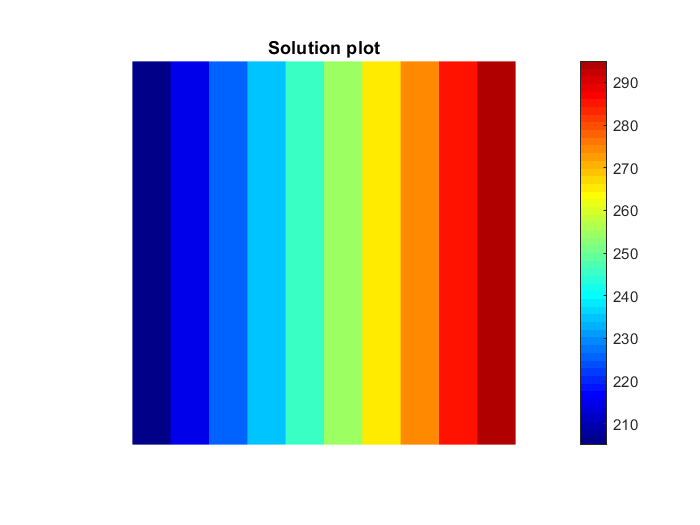
\includegraphics[width=1\linewidth]{figs/diffusion_default_simulation}
		\caption{2D plot of computational domain with colormap of $ \phi $ in cell centers.}
		\label{fig:diffusiondefaultsimulation}
	\end{subfigure}
	\begin{subfigure}{.49\textwidth}
		\centering
		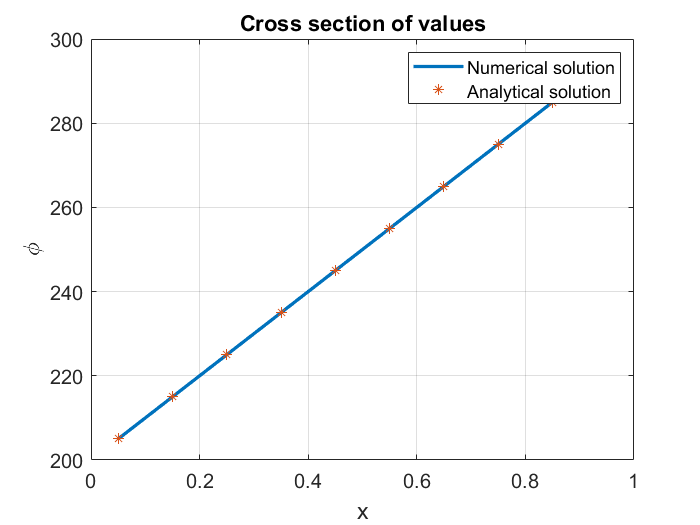
\includegraphics[width=1\linewidth]{figs/diffusion_default_cross}
		\caption{Cross section for $ y = const.$ Plotted are values in cell centers.}
		\label{fig:diffusiondefaultcross}
	\end{subfigure}
	\caption{Basic diffusion test case.}
	\label{fig:diffusion_default}
\end{figure}

\subsubsection{Cold plate}
This test case is also defined on a square domain, but with all boundaries of Dirichlet type and value of $ \phi^D $ except for ther northern wall, where it is set different. Such case has an analytical solution in form of an endless sum
\begin{equation}
\phi(x,y) = T_1 + (T2-T1) \cdot \dfrac{2}{\pi} \cdot \sum_{n=1}^{\infty} \dfrac{(-1)^{n+1}+1}{n} \cdot \sin\left(\dfrac{n\pi x}{L}\right) \cdot \dfrac{\sinh\left(\dfrac{n\pi y}{W}\right)}{\sinh\left(\dfrac{n\pi H}{L}\right)},
\end{equation}

which was for the purpose of computational purposes cut off at $ n=800 $. This means that even though we have an analytical formula, the solution is not exact, but still taken as reference. Also the boundary conditions do not satisfy the condition of agreement ($ T_1 \neq T_2 $) in the north-west and north-east corner which leads to bigger disagreement between the numerical and analytical solution in these parts.



\begin{figure}
	\centering
	\begin{subfigure}{.49\textwidth}
		\centering
		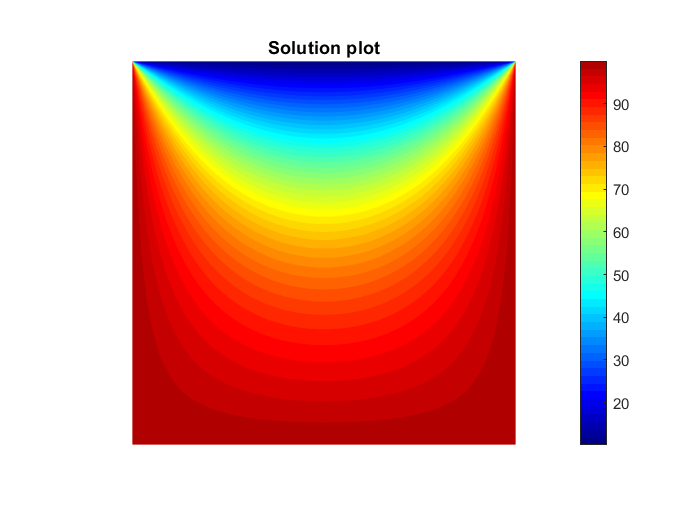
\includegraphics[width=1\linewidth]{figs/diffusion_hot_plate_simulation_1k}
		\caption{2D plot of computational domain with colormap of $ \phi $ in cell centers.}
		\label{fig:diffusionhotplatesimulation1k}
	\end{subfigure}
	\begin{subfigure}{.49\textwidth}
		\centering
		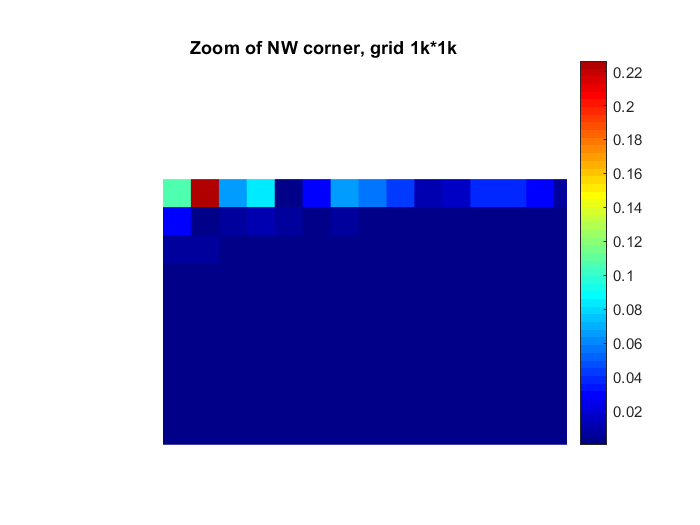
\includegraphics[width=1\linewidth]{figs/diffusion_hot_plate_error_corner_1k}
		\caption{Relative error of numerical solution, zoom of north-western corner.}
		\label{fig:diffusionhotplateerrorcorner1k}
	\end{subfigure}
	\caption{Cold plate diffusion test case.}
	\label{fig:diffusion_hot_plate}
\end{figure}


\begin{table}
	\centering
	\begin{tabular}{|c|c|c|}
		\hline
		grid cells & $ \epsilon_{max} $ & $ \epsilon_{mean} $\\
		\hline
		10*10 & 6.7966 e-02 & 4.7048 e-03 \\
		\hline
		100*100 &  6.9899 e-02 & 1.0538 e-04 \\
		\hline
		1k*1k & 2.2625 e-01 & 8.1376 e-06 \\
		\hline
	\end{tabular}
	\caption{Maximum and average relative error for cold plate test case when refining grid.}
	\label{tab:diffusion_hot_plate_grid}
\end{table}

The Figure \ref{fig:diffusion_hot_plate} presents the final solution of this test case for grid of $ 1000*1000 $ cells. As already mentioned, when comparing the results to analytical solution, the biggest disagreement is in the corners. This is demonstrated on the figure \ref{fig:diffusionhotplateerrorcorner1k}, which shows the northe-western corner of computational domain with colormap of the relative error $ \epsilon $ computed in all cells separately using 
\begin{equation}
\epsilon = \dfrac{|\phi_{num}-\phi_{anal}|}{|\phi_{anal}|}.
\end{equation}
Due to these singularities, the maximum relative error actually grows when refining the grid as shown in Table \ref{tab:diffusion_hot_plate_grid}, but the average relative arror goes down as one would expect. 


\section{Convection-diffusion}
The governing equation for this part is 
\begin{equation}\label{eq:convection}
(\mathbf{u} \cdot \nabla)\phi - \nabla \cdot (\kappa\nabla\phi) = S_\phi,
\end{equation}
where $ \phi $ represents a scalar quantity, $ S_\phi $ volume source, $ \kappa $ a diffusivity coefficient and $ \mathbf{u} $ a vector of velocity.

\subsection{Discretization process} \label{subsec:conv_disc}
By applying the same procedure as in previous chapter and ignoring the volume source term for now, we can transform equation \ref{eq:convection} into
\begin{equation}\label{key}
\int_{\Gamma} \mathbf{u\cdot n}\phi \, ds - \int_\Gamma \kappa \nabla \phi \cdot n \, ds = 0.
\end{equation}
Again making the assumption of orthogonal square grid and using mean values to represent integrals over each face (parts of $ \Gamma $), we can replace the integrals with a sum
\begin{equation}
\sum_{\forall f} u_{n,f}\phi_f A_f - \sum_{\forall f} \kappa  \left(\frac{\partial\phi}{\partial n}\right)_f A_f = 0,
\end{equation} 
where $ u_{n,f} $ denotes the product of $ \mathbf{u} $ in center of face $ f $ and normal vector $ \mathbf{n} $ of that face. This value is interpolated for said grid of cells as 
\begin{equation}
u_{n,f} = \dfrac{\mathbf{u}_{nb1}+\mathbf{u}_{nb2}}{2}\cdot \mathbf{n}_f,
\end{equation}
where again $ nb1 $ and $ nb2 $ denote the cells sharing $ f $. For unequally sized cells, a different formula should be used. 

With this, the equation for one grid cell changes into
\begin{equation}\label{eq:convection_one_cell}
a_P\phi_P + \sum_{nb} a_{nb} \phi_{nb} =0,
\end{equation}
where
\begin{align}
a_P &= a_P^{conv} + a_P^{diff},\,
a_{nb} = a_{nb}^{conv} + a_{nb}^{diff},\\
a_P^{diff} &= - \sum_{nb} a_{nb}^{diff},\,
a_{nb}^{diff} = \kappa \dfrac{A_f}{||\boldsymbol{\xi}_f||},\\
a_P^{conv} &=  - \sum_{nb} a_{nb}^{conv},\,
a_{nb}^{conv} = A_f \cdot \dfrac{u_{n,f}}{2}, \, f = P \cap nb.
\end{align}

This, together with the same implementation of boundary conditions allows to construct a system of linear equations, that gives an approximate solution to governing equation \ref{eq:convection}.

\subsection{Verification}
For the verification of convection-diffusion, the results of simulation were compared to a single analyticaly solvable test case.
\subsubsection{Convection diffusion test case}
This test case is again defined on a square domain, with adiabatic boundary conditions on north and south walls and Dirichlet condition on west and east boundaries with different values of $ \phi^D $. The velocity field $ \mathbf{u} = \left( u_x, u_y\right) $ is set uniformly over the whole domain to $ \left( 50,0\right) $. The analytical solution to this case is independent of $ y $ and can be written as 
\begin{equation}\label{eq:convection_anal}
\phi(x) = T_1 + (T_2 - T_1) \dfrac{\exp\left(\dfrac{P\cdot x 	}{L}-1\right)}{\exp\left(P\right)-1},\, P = \dfrac{u_x \cdot L}{\kappa},
\end{equation}
where $ T_1 $ and $ T_2 $ are values of Dirichlet boundary conditions on west and east wall respectively.

To compare the results of simulation to the analytical solution a cross section of constant $ y $ is done through the domain and the values in cell centers are compared to analytical solution as shown in figure \ref{fig:convectiondiffusioncross10}. The relative error between these solutions is again computed in the same manner as in equation \ref{eq:diffusion_relerror} and its values for different refined grids are shown in Table \ref{tab:convection_diffusion_grid}, proving grid convergence for this test case. Figure \ref{fig:convectiondiffusion} then gives the big picture by showing of $ \phi $ over the whole domain for the simulation with the finest mesh.

\begin{figure}
	\centering
	\begin{subfigure}{.49\textwidth}
		\centering
		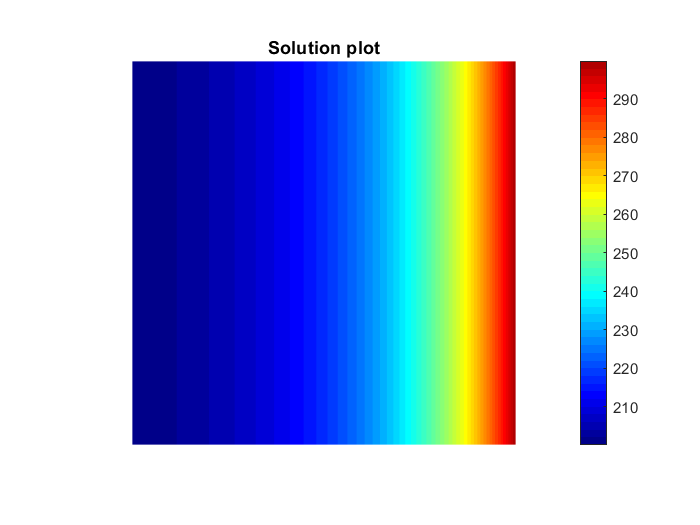
\includegraphics[width=1\linewidth]{figs/convection_diffusion}
		\caption{2D plot of computational domain with colormap of $ \phi $. Grid of 1000*1000 cells}
		\label{fig:convectiondiffusion}
	\end{subfigure}
	\begin{subfigure}{.49\textwidth}
		\centering
		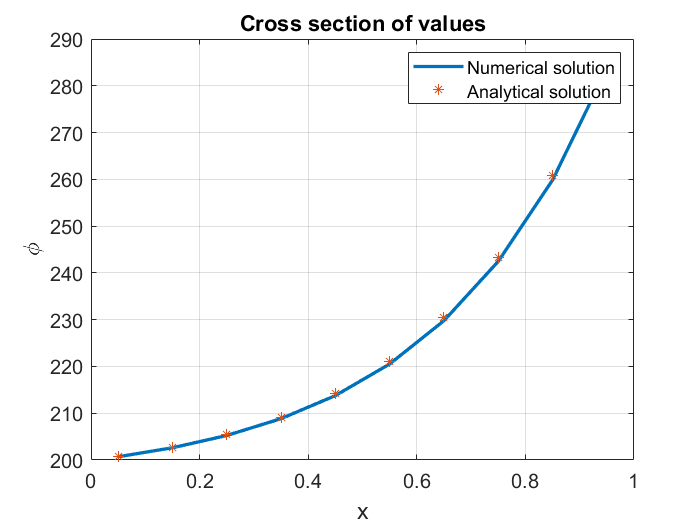
\includegraphics[width=1\linewidth]{figs/convection_diffusion_cross_10}
		\caption{Cross section for $y=const.$ and grid of 10*10 cells.}
		\label{fig:convectiondiffusioncross10}
	\end{subfigure}
	\caption{Test case for convection-diffusion.}
	\label{fig:convection_test_case}
\end{figure}


\begin{table}
	\centering
	\begin{tabular}{|c|c|}
		\hline
		grid cells & $ \epsilon $ \\
		\hline
		10*10 &2.8045 e-03  \\
		\hline
		100*100 &  2.8003 e-05  \\
		\hline
		1k*1k & 2.8003 e-07 \\
		\hline
	\end{tabular}
	\caption{Convergence of relative error when refining grid.}
	\label{tab:convection_diffusion_grid}
\end{table}

\subsection{Rotated grid}
The implementation of both convection and diffusion are applicable also for rotated grids. This is not discussed in much detail but a visual proof of this is shown in Figure \ref{fig:convectiondiffusionrotated}.
\begin{figure}
	\centering
	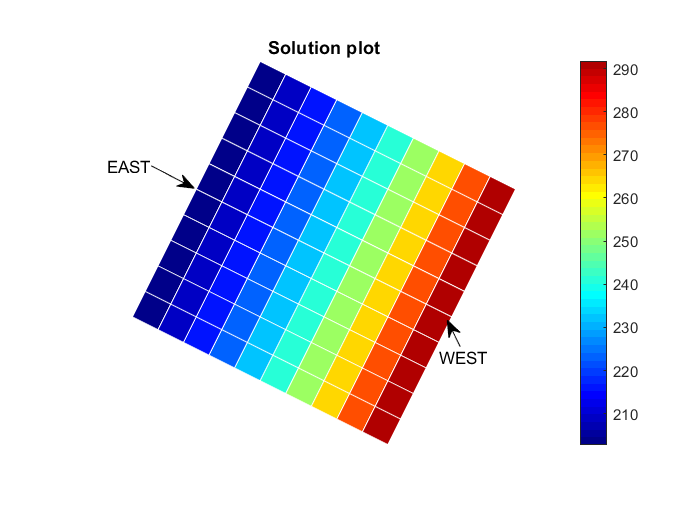
\includegraphics[width=0.8\linewidth]{figs/convection_diffusion_rotated}
	\caption{Convection-diffusion on rotated grid.}
	\label{fig:convectiondiffusionrotated}
\end{figure}




\section{Fixed pressure momentum equation}
The governing equation for this part is 
\begin{equation}\label{eq:pressure_momentum}
\dfrac{\partial \mathbf{u}}{\partial t} + (\mathbf{u} \cdot \nabla)\mathbf{u} = \nabla \cdot (\nu\nabla\mathbf{u}) - \dfrac{1}{\rho}\nabla p,
\end{equation}
where $ \mathbf{u} $ represents a vector of velocity, $ t $ is time, $ \nu $ a diffusivity coefficient, $ \rho $ density of the transport medium and $ \nabla p $ pressure gradient. 

\subsection{Discretization}

Although the resulting solutions are expected to be steady state, the first term containing time partial derivative w.r.t. time is kept and used to linearize the equations (equation \ref{eq:pressure_momentum} is a vector equation), because the term $ (\mathbf{u} \cdot \nabla)\mathbf{u} $ is non-linear. For the time discretization an implicit Euler scheme will be used, thus one $ \mathbf{u} $ from the non-linear term will be taken from current time layer, while the other from the future one.

By integrating the governing equation over control volume and applying the Gauss theorem we arrive to 
\begin{equation}\label{eq:pressure_momentum_integral}
\int_{CV} \dfrac{\partial \mathbf{u}}{\partial t} \, d\Omega + \int_{\Gamma} (\mathbf{u\cdot n})\mathbf{u} \, ds = \int_{\Gamma} \nu \mathbf{n \cdot \nabla u} \, ds - \int_{CV} \dfrac{1}{\rho}\nabla p \, d \Omega.
\end{equation}
Again replacing the integrals using mean values over their respective integration areas and assuming $ \nabla p $ constant throughout the control volume we can write a semi-discretized equation (time derivative is still present) 
\begin{equation}\label{eq:pressure_momentum_semi_discrete}
\dfrac{\partial \mathbf{u}}{\partial t} \Omega_{cell} + \sum_{\forall f} u_{n,f} \mathbf{u_f} A_f = \sum_{\forall f}\nu \left(\dfrac{\partial \mathbf{u}}{\partial n}\right)_f A_f - \dfrac{1}{\rho} \nabla p \Omega_{cell}
\end{equation}
and discretizing in time as well by applying Euler implicit time discretization scheme
\begin{equation}
 \dfrac{\partial \mathbf{u}}{\partial t} \approx \dfrac{\mathbf{u^{N+1} - u^{N} }}{\Delta t} = \mathbf{F(u^{N+1})},
\end{equation} 
equation \ref{eq:pressure_momentum_semi_discrete} transforms to
\begin{equation}
\dfrac{\mathbf{u^{N+1} - u^{N} }}{\Delta t} \Omega_{cell}+ \sum_{\forall f} u_{n,f}^{\mathbf{N}} \mathbf{u^{N+1}}_f A_f = \sum_{\forall f}\nu \left(\dfrac{\partial \mathbf{u^{N+1}}}{\partial n}\right)_f A_f - \dfrac{1}{\rho} \nabla p \Omega_{cell},
\end{equation}
which gives a system of equations $ \mathbf{A}\cdot\mathbf{u^{N+1}} = \mathbf{b} $.
For a 2D case, the vector $ \mathbf{u} $ has only two components $ u_x,\,u_y $ and equations for both of these parts are decoupled, meaning that we can solve $ \mathbf{A}_x\cdot u_x = \mathbf{b}_x $ and $ \mathbf{A}_y \cdot u_y = \mathbf{b}_y $ separately and put the results together to get $ \mathbf{u}$. For simplicity sake, the parts of the linear equaitons system are still expressed in vector form and getting the $ x $ or $ y $ component from these is trivial. The equations for a single cell $ P $ compose of
\begin{align}
\mathbf{b}_P &= \dfrac{\mathbf{u}^N_P}{\Delta t} \Omega_{P}- \dfrac{1}{\rho} \nabla p_P \cdot \Omega_P,\\
\mathbf{a}_P &= \mathbf{a}_{P}^{time} + \mathbf{a}_{P}^{conv} +\mathbf{a}_{P}^{diff}, \\
\mathbf{a}_{P}^{time}&=\mathbf{e}\dfrac{1}{\Delta t}\Omega_P,
\end{align}
with $ \mathbf{a}_{P}^{conv}, \mathbf{a}_{P}^{diff} $ constructed in the same manner as in section \ref{subsec:conv_disc}.

\subsection{Verification}
To verify correctness of implementation a single analytically solvable test case was implemented and compared to results of simulation. Also \textbf{method of manufactured solutio}n was applied to check the correctness of the code. The total tolerance was set to $ 10^{-9} $ and time step $ \Delta t = 50 $.

\subsubsection{Combined pressure and lid driven flow}
The test case is defined as flow between two plates of length $ L=1\,m $ and width $ W $ with a gap between them of size $ H=1\,m $. The top plate is moving in direction of $ x $-axis with speed $ U = 5\, m\cdot s^{-1} $ and the pressure difference between beginning and end of computational domain is $ \Delta p = 100\, Pa $. Properties of the transported fluid are $ \nu = 0.15 \, m^2\cdot s^{-1} $ and $ \rho=10 \,kg\cdot m^{-3} $, which probably does not correspond to any real fluid but for verification it is important that the values are $ \neq 1 $ to really see if their influence propagates in the simulation. 

This case can be solved analytically by superposing two well known cases of pressure driven (Figure \ref{fig:pressuredrivenflow}) and lid driven (Figure \ref{fig:liddrivenflow}) flow. Only non-zero component of $ \mathbf{u} $ is $ u_x $ for which we can write 
\begin{equation}\label{eq:pressure_lid_analytical}
u_x(y)= \underbrace{\dfrac{1}{2}\dfrac{\Delta p \cdot H^2}{\nu\cdot \rho} \left[ \left(\dfrac{y}{H}\right)^2 - \dfrac{y}{H} \right] }_{pressure\, driven \, flow} + \underbrace{U \cdot \dfrac{y}{H}}_{lid \,driven \,flow}. 
\end{equation}

To compare the results of simulation, a cross section for constant $ x $ is made through the computational domain as shown on Figure \ref{fig:pressuredrivenflowcross10} and error of the solution is computed in the same manner as in equation \ref{eq:diffusion_relerror}. The values of $ \epsilon $ for differently refined grids are displayed in Table \ref{tab:pressure_momentum_grid} and show signs of convergence, reaching error in magnitude of total tolerance set in the code. Since velocity in $ y $ direction is zero, the Figure \ref{fig:pressuredrivenflow} shows only the $ x $-component of $ \mathbf{u} $. Outputs produced by the simulation technique show good agreement with analytical solution and so the implementation may be considered validated.

\begin{figure}
	\centering
	\begin{subfigure}{.49\textwidth}
		\centering
		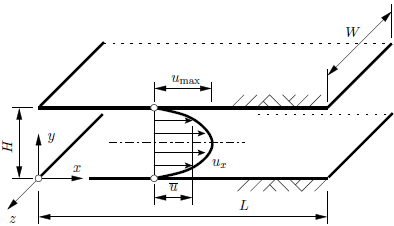
\includegraphics[width=1\linewidth]{figs/pressure_driven_flow}
		\caption{Illustration of pressure driven flow between two plates.}
		\label{fig:pressuredrivenflow}
	\end{subfigure}
	\begin{subfigure}{.49\textwidth}
		\centering
		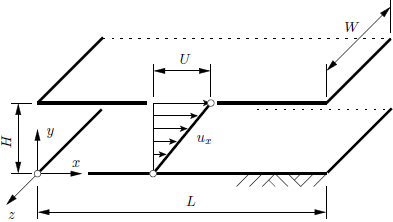
\includegraphics[width=1\linewidth]{figs/lid_driven_flow}
		\caption{Illustration of lid driven flow between two plates.}
		\label{fig:liddrivenflow}
	\end{subfigure}
	\caption{Test case illustrative images. Images taken from study materials from course Transport of Momentum, Heat and Mass at CTU Prague.}
	\label{fig:pressure_and_lid_driven_ilustartion}
\end{figure}

\begin{table}
	\centering
	\begin{tabular}{|c|c|}
		\hline
		grid cells & $ \epsilon $ \\
		\hline
		10*10 & 9.7355e-03  \\
		\hline
		100*100 & 9.7434e-05  \\
		\hline
		1k*1k & 9.4675e-07 \\
		\hline
		10*10k & 9.7417e-09 \\
		\hline
	\end{tabular}
	\caption{Convergence of relative error when refining grid.}
	\label{tab:pressure_momentum_grid}
\end{table}

\begin{figure}
	\centering
	\begin{subfigure}{.49\textwidth}
		\centering
		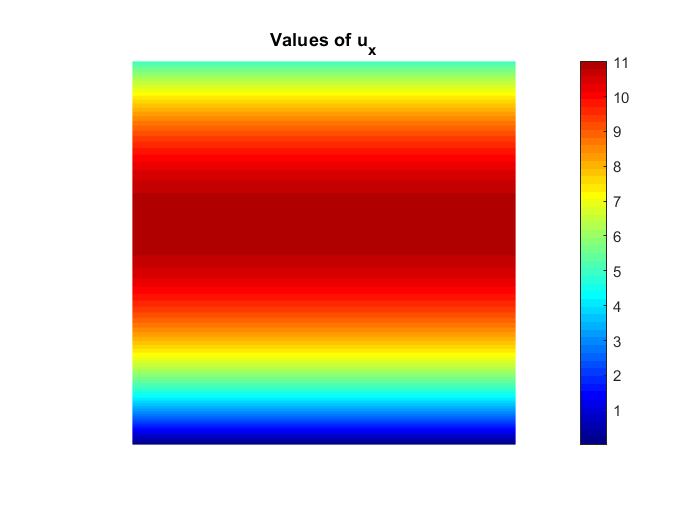
\includegraphics[width=1\linewidth]{figs/pressure_lid_flow}
		\caption{Colormap of $u_x$ velocity component within computational domain.}
		\label{fig:pressurelidflow}
	\end{subfigure}
	\begin{subfigure}{.49\textwidth}
		\centering
		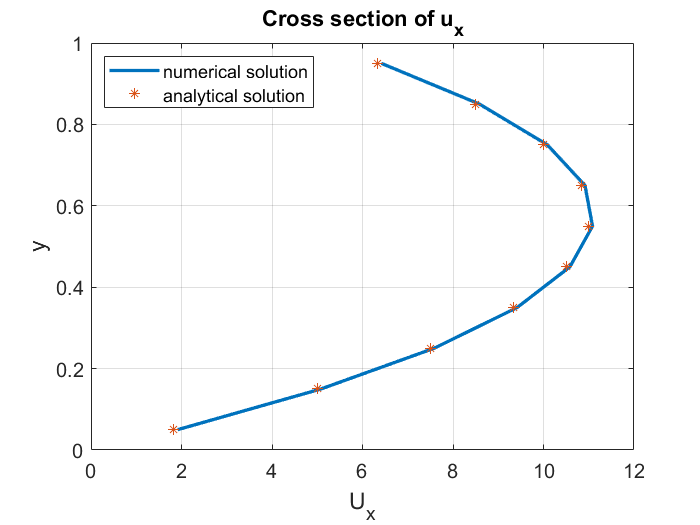
\includegraphics[width=1\linewidth]{figs/pressure_driven_flow_cross10}
		\caption{Comparisson of numerical and analytical solution in a cross section for constant $x$.}
		\label{fig:pressuredrivenflowcross10}
	\end{subfigure}
	\caption{Test case for fixed pressure momentum implementation - pressure and lid driven flow.}
	\label{fig:pressure_and_lid_flow_figs}
\end{figure}

\subsubsection{Method of manufactured solutions}
The second way how to verify the implementation is method of manufactured solution. Here we take an arbitrary solution (which does not necessarily have to be physical) and derive source terms which will be used in the simulation. If everything is correct in the implementation, then the results of the simulation should be equal to the chosen arbitrary solution.

The chosen solution for which this test was perforemed is 
\begin{equation}\label{eq:MMS_arbitrary_solution}
\mathbf{u}(x,y) = x^2 \cdot \mathbf{e}_x - y^2 \cdot \mathbf{e}_y.
\end{equation}
Plugging this solution into steady-state momentum equation with sources
\begin{align}
\dfrac{\partial u u}{\partial x} + \dfrac{\partial u v}{\partial y} - \left( \dfrac{\partial}{\partial x}\nu\dfrac{\partial u}{\partial x} + \dfrac{\partial}{\partial y}\nu \dfrac{\partial u}{\partial y} \right) &= S_x, \\
\dfrac{\partial u v}{\partial x} + \dfrac{\partial v v}{\partial y} - \left( \dfrac{\partial}{\partial x}\nu\dfrac{\partial v}{\partial x} + \dfrac{\partial}{\partial y}\nu \dfrac{\partial v}{\partial y} \right) &= S_y,
\end{align}
which is equation \ref{eq:pressure_momentum} without time dependent term and with arbitrary source term $ \mathbf{S} = \left[ S_x, S_y \right] $ instead of pressure gradient source, we arrive to
\begin{align}
S_x& = 4x^3 - 2x^2y -2 \nu, \\
S_y& = -2xy^2 + 4y^3 +2 \nu.
\end{align}
The solution in equation \ref{eq:MMS_arbitrary_solution} is then also used determine the coefficients for boundary conditions of both Neumann (west and east boundaries) and Dirichlet type (north and south).

Figure \ref{fig:mmssolution} show the prescribed vectors of velocity on faces with colormap of $ u_x $ component. The absolute difference in solution and simulation for both components of velocity is shown in Figures \ref{fig:MMS_differences}. The table \ref{tab:MMS_grid} shows relative error for different grids 

\begin{figure}
	\centering
	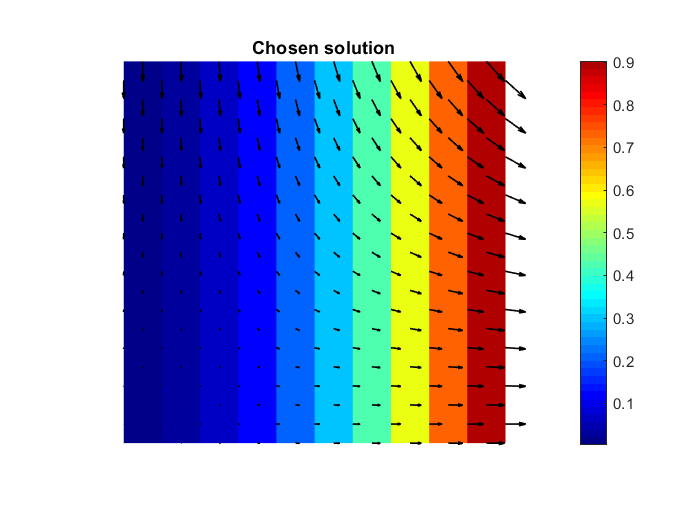
\includegraphics[width=0.7\linewidth]{figs/MMS_solution}
	\caption{Chosen solution $ \mathbf{u} $ for validation using MMS.}
	\label{fig:mmssolution}
\end{figure}

\begin{figure}
	\centering
	\begin{subfigure}{.49\textwidth}
		\centering
		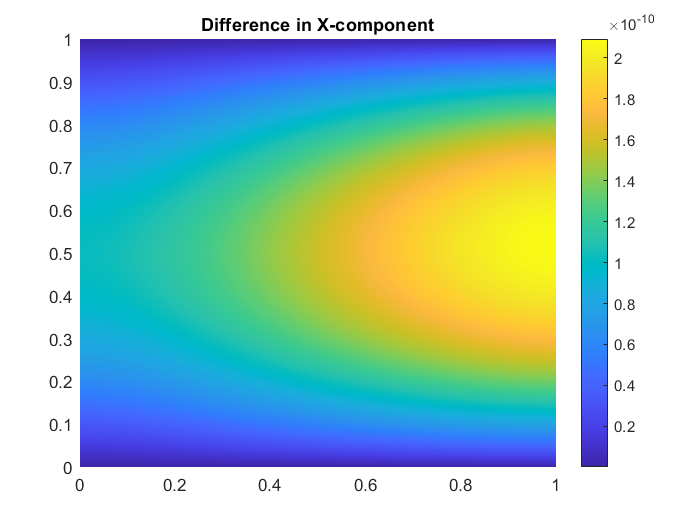
\includegraphics[width=1\linewidth]{figs/MMS_xdiff}
		\caption{Absolute difference in $ u_x^{chosen} $ and $ u_x^{simulation} $.}
		\label{fig:mmsxdiff}
	\end{subfigure}
	\begin{subfigure}{.49\textwidth}
		\centering
		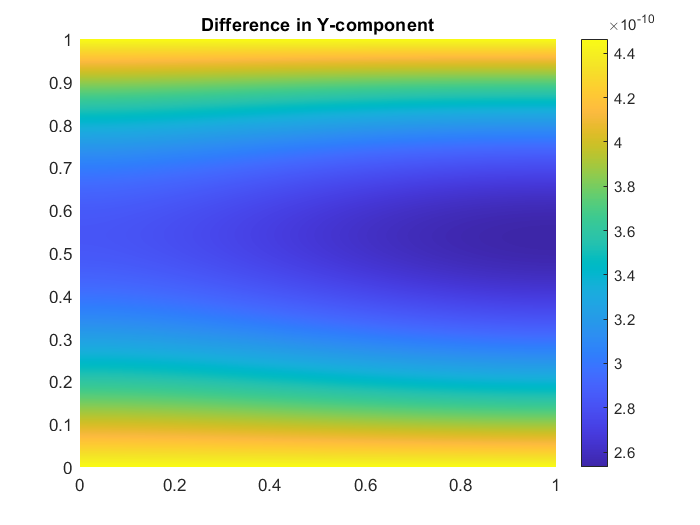
\includegraphics[width=1\linewidth]{figs/MMS_ydiff}
		\caption{Absolute difference in $ u_y^{chosen} $ and $ u_y^{simulation} $.}
		\label{fig:mmsydiff}
	\end{subfigure}
	\caption{Absolute errors in both components of velocity $ \mathbf{u} $ for mesh with 1k*1k cells.}
	\label{fig:MMS_differences}
\end{figure}



\begin{table}
	\centering
	\begin{tabular}{|c|c|}
		\hline
		grid cells & $ \epsilon $ \\
		\hline
		10*10 & 3.3183e-03  \\
		\hline
		100*100 & 3.5344e-05  \\
		\hline
		1k*1k & 3.3590e-07 \\
		\hline
	\end{tabular}
	\caption{Convergence of relative error when refining grid.}
	\label{tab:MMS_grid}
\end{table}


\end{document}